% Generated by code/needham.py -- do not edit by hand.
\definecolor{qocA}{rgb}{0.00,0.45,0.70}
\definecolor{qocB}{rgb}{0.90,0.60,0.00}
\definecolor{qocC}{rgb}{0.00,0.62,0.45}
\definecolor{qocD}{rgb}{0.80,0.40,0.00}
\definecolor{qocE}{rgb}{0.80,0.60,0.70}
\definecolor{qocF}{rgb}{0.35,0.70,0.90}
\begin{tikzpicture}[ink/.style={line width=0.9pt, ndInk}, faint/.style={line width=0.4pt, ndInk!35}, dashedink/.style={line width=0.5pt, ndInk!55, dash pattern=on 2.5pt off 2pt}, vec/.style={->, >=stealth, line width=1.2pt}, note/.style={font=\footnotesize\itshape, text=ndInk!85, align=center}, pointer/.style={->, >=stealth, line width=0.4pt, ndInk!60, shorten >=2pt, shorten <=1pt}, dot/.style={circle, fill=ndInk, inner sep=0pt, minimum size=3.4pt}, wash/.style={fill=ndSky, fill opacity=0.55}, every node/.style={text=ndInk}]
\definecolor{ndInk}{rgb}{0.13,0.13,0.18}
\definecolor{ndPaper}{rgb}{0.99,0.96,0.88}
\definecolor{ndSky}{rgb}{0.84,0.91,0.98}
\definecolor{ndRose}{rgb}{0.98,0.86,0.84}
\definecolor{ndBlue}{rgb}{0.13,0.36,0.66}
\definecolor{ndRed}{rgb}{0.78,0.20,0.16}
\definecolor{ndGold}{rgb}{0.88,0.62,0.10}
\definecolor{ndGreen}{rgb}{0.18,0.52,0.30}
\fill[ndBlue!18] (4.804,2.600) rectangle (7.396,3.420);
\fill[ndRed!18] (5.184,2.600) rectangle (7.016,1.780);
\draw[faint, ->, >=stealth] (0.292,2.600) -- (14.614,2.600) node[right, text=ndInk, font=\small] {$\nu$};
\draw[faint] (6.100,2.520) -- (6.100,2.680);
\draw[line width=1.1pt, ndBlue] (2.896,2.600) -- (2.896,3.300);
\draw[ndBlue, line width=0.7pt, fill=white] (2.896,3.300) circle (1.6pt);
\draw[line width=1.1pt, ndBlue] (5.488,2.600) -- (5.488,3.300);
\fill[ndBlue] (5.488,3.300) circle (2.0pt);
\draw[line width=1.1pt, ndBlue] (8.080,2.600) -- (8.080,3.300);
\draw[ndBlue, line width=0.7pt, fill=white] (8.080,3.300) circle (1.6pt);
\draw[line width=1.1pt, ndBlue] (10.672,2.600) -- (10.672,3.300);
\draw[ndBlue, line width=0.7pt, fill=white] (10.672,3.300) circle (1.6pt);
\draw[line width=1.1pt, ndBlue] (13.264,2.600) -- (13.264,3.300);
\draw[ndBlue, line width=0.7pt, fill=white] (13.264,3.300) circle (1.6pt);
\draw[line width=1.1pt, ndRed] (0.749,2.600) -- (0.749,1.900);
\draw[ndRed, line width=0.7pt, fill=white] (0.749,1.900) circle (1.6pt);
\draw[line width=1.1pt, ndRed] (2.582,2.600) -- (2.582,1.900);
\draw[ndRed, line width=0.7pt, fill=white] (2.582,1.900) circle (1.6pt);
\draw[line width=1.1pt, ndRed] (4.415,2.600) -- (4.415,1.900);
\draw[ndRed, line width=0.7pt, fill=white] (4.415,1.900) circle (1.6pt);
\draw[line width=1.1pt, ndRed] (6.247,2.600) -- (6.247,1.900);
\fill[ndRed] (6.247,1.900) circle (2.0pt);
\draw[line width=1.1pt, ndRed] (8.080,2.600) -- (8.080,1.900);
\draw[ndRed, line width=0.7pt, fill=white] (8.080,1.900) circle (1.6pt);
\draw[line width=1.1pt, ndRed] (9.913,2.600) -- (9.913,1.900);
\draw[ndRed, line width=0.7pt, fill=white] (9.913,1.900) circle (1.6pt);
\draw[line width=1.1pt, ndRed] (11.745,2.600) -- (11.745,1.900);
\draw[ndRed, line width=0.7pt, fill=white] (11.745,1.900) circle (1.6pt);
\draw[line width=1.1pt, ndRed] (13.578,2.600) -- (13.578,1.900);
\draw[ndRed, line width=0.7pt, fill=white] (13.578,1.900) circle (1.6pt);
\draw[ndGold, line width=1.6pt] (8.080,2.600) circle (5pt);
\node[font=\small, text=ndBlue, anchor=east] at (0.274,3.020) {$\tau_1=1.6$};
\node[font=\small, text=ndRed, anchor=east] at (0.274,2.180) {$\tau_2=\sqrt2\,\tau_1$};
\fill[ndBlue!18] (4.804,-1.000) rectangle (7.396,-0.180);
\fill[ndRed!18] (5.236,-1.000) rectangle (6.964,-1.820);
\draw[faint, ->, >=stealth] (0.292,-1.000) -- (14.614,-1.000) node[right, text=ndInk, font=\small] {$\nu$};
\draw[faint] (6.100,-1.080) -- (6.100,-0.920);
\draw[line width=1.1pt, ndBlue] (2.896,-1.000) -- (2.896,-0.300);
\draw[ndBlue, line width=0.7pt, fill=white] (2.896,-0.300) circle (1.6pt);
\draw[line width=1.1pt, ndBlue] (5.488,-1.000) -- (5.488,-0.300);
\fill[ndBlue] (5.488,-0.300) circle (2.0pt);
\draw[line width=1.1pt, ndBlue] (8.080,-1.000) -- (8.080,-0.300);
\draw[ndBlue, line width=0.7pt, fill=white] (8.080,-0.300) circle (1.6pt);
\draw[line width=1.1pt, ndBlue] (10.672,-1.000) -- (10.672,-0.300);
\draw[ndBlue, line width=0.7pt, fill=white] (10.672,-0.300) circle (1.6pt);
\draw[line width=1.1pt, ndBlue] (13.264,-1.000) -- (13.264,-0.300);
\draw[ndBlue, line width=0.7pt, fill=white] (13.264,-0.300) circle (1.6pt);
\draw[line width=1.1pt, ndRed] (1.168,-1.000) -- (1.168,-1.700);
\draw[ndRed, line width=0.7pt, fill=white] (1.168,-1.700) circle (1.6pt);
\draw[line width=1.1pt, ndRed] (2.896,-1.000) -- (2.896,-1.700);
\draw[ndRed, line width=0.7pt, fill=white] (2.896,-1.700) circle (1.6pt);
\draw[line width=1.1pt, ndRed] (4.624,-1.000) -- (4.624,-1.700);
\draw[ndRed, line width=0.7pt, fill=white] (4.624,-1.700) circle (1.6pt);
\draw[line width=1.1pt, ndRed] (6.352,-1.000) -- (6.352,-1.700);
\fill[ndRed] (6.352,-1.700) circle (2.0pt);
\draw[line width=1.1pt, ndRed] (8.080,-1.000) -- (8.080,-1.700);
\draw[ndRed, line width=0.7pt, fill=white] (8.080,-1.700) circle (1.6pt);
\draw[line width=1.1pt, ndRed] (9.808,-1.000) -- (9.808,-1.700);
\draw[ndRed, line width=0.7pt, fill=white] (9.808,-1.700) circle (1.6pt);
\draw[line width=1.1pt, ndRed] (11.536,-1.000) -- (11.536,-1.700);
\draw[ndRed, line width=0.7pt, fill=white] (11.536,-1.700) circle (1.6pt);
\draw[line width=1.1pt, ndRed] (13.264,-1.000) -- (13.264,-1.700);
\draw[ndRed, line width=0.7pt, fill=white] (13.264,-1.700) circle (1.6pt);
\draw[ndGold, line width=1.6pt] (2.896,-1.000) circle (5pt);
\draw[ndGold, line width=1.6pt] (8.080,-1.000) circle (5pt);
\draw[ndGold, line width=1.6pt] (13.264,-1.000) circle (5pt);
\node[font=\small, text=ndBlue, anchor=east] at (0.274,-0.580) {$\tau_1=1.6$};
\node[font=\small, text=ndRed, anchor=east] at (0.274,-1.420) {$\tau_2=\tfrac32\,\tau_1$};
\node[font=\scriptsize, anchor=north west, inner sep=1pt] at (8.200,2.550) {$\omega$};
\node[font=\scriptsize, anchor=north east, inner sep=1pt] at (6.060,2.550) {$0$};
\node[font=\scriptsize, anchor=north west, inner sep=1pt] at (8.200,-1.050) {$\omega$};
\node[font=\scriptsize, anchor=north east, inner sep=1pt] at (6.060,-1.050) {$0$};
\node[note, anchor=south] (g) at (8.080,3.550) {the only tooth common to both combs:\\ the true frequency $\omega$};
\draw[pointer] (g.south) -- (8.260,2.820);
\node[note, anchor=south] (fb) at (2.602,3.550) {filled dots: the tooth each rate reports\\ on its own, in its Nyquist band (shaded)};
\draw[pointer] (fb.south east) to[bend left=10] (5.428,3.360);
\node[note, anchor=west] at (15.066,2.600) {spacing $2\pi/\tau_1$ (up)\\ and $2\pi/\tau_2$ (down):\\ irrational ratio};
\node[note, anchor=west] at (15.066,-1.000) {rational ratio: the\\ combs coincide\\ every $4\pi/\tau_1$};
\node[note, anchor=north, text=ndInk] (amb) at (8.080,-1.950) {three candidates remain in the window, and the ambiguity persists};
\draw[pointer] (amb.north) -- (2.846,-1.220);
\draw[pointer] (amb.north) -- (8.080,-1.220);
\draw[pointer] (amb.north) -- (13.314,-1.220);
\node[font=\small] at (7.420,1.350) {(a) irrational ratio of the sampling periods};
\node[font=\small] at (7.420,-2.850) {(b) rational ratio of the sampling periods};
\end{tikzpicture}
